\documentclass[border=4pt]{standalone}
% Shared typography and colours for the standalone figures.
\usepackage{unicode-math}
\setmainfont{TeX Gyre Termes}
\setmathfont{TeX Gyre Termes Math}
\usepackage{tikz}
\usetikzlibrary{arrows.meta,positioning,calc,decorations.pathreplacing}
\usepackage{pgfplots}
\pgfplotsset{compat=1.18}
% Stored subsystem, transfer channel, driver, and internal observation.
\definecolor{elemA}{HTML}{1F5FA8}
\definecolor{elemB}{HTML}{B8461B}
\definecolor{elemC}{HTML}{2E7D32}
\definecolor{elemD}{HTML}{6A4C93}
\definecolor{frameline}{HTML}{555555}

\begin{document}
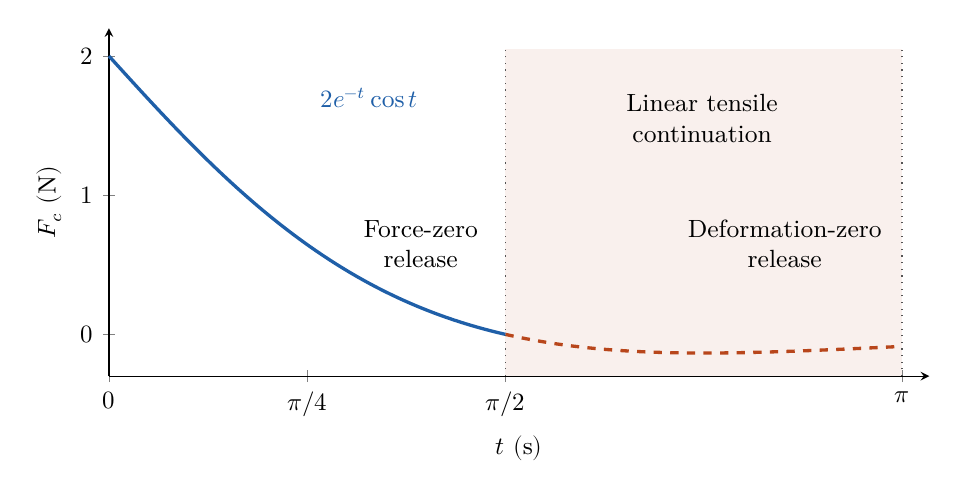
\begin{tikzpicture}
\begin{axis}[width=12cm,height=6cm,xmin=0,xmax=3.25,ymin=-.3,ymax=2.2,
 axis lines=left,xlabel={$t\ (\mathrm s)$},ylabel={$F_c\ (\mathrm N)$},
 xtick={0,.7853981634,1.570796327,3.141592654},
 xticklabels={$0$,$\pi/4$,$\pi/2$,$\pi$},ytick={0,1,2},
 tick label style={font=\small},label style={font=\small},clip=false]
\path[fill=elemB!8] (axis cs:1.570796327,-.3) rectangle (axis cs:3.141592654,2.05);
\addplot[elemA,very thick,domain=0:1.570796327,samples=100] {2*exp(-x)*cos(deg(x))};
\addplot[elemB,very thick,dashed,domain=1.570796327:3.141592654,samples=100] {2*exp(-x)*cos(deg(x))};
\draw[dotted,frameline] (axis cs:1.570796327,-.3) -- (axis cs:1.570796327,2.05);
\draw[dotted,frameline] (axis cs:3.141592654,-.3) -- (axis cs:3.141592654,2.05);
\node[align=center,font=\small] at (axis cs:2.35,1.55) {Linear tensile\\continuation};
\node[align=left,font=\small,anchor=west,elemA] at (axis cs:.8,1.7) {$2e^{-t}\cos t$};
\node[align=center,font=\small,anchor=east] at (axis cs:1.5,.65) {Force-zero\\release};
\node[font=\small,align=center,anchor=east] at (axis cs:3.1,.65) {Deformation-zero\\release};
\end{axis}
\end{tikzpicture}
\end{document}
